\documentclass[12pt,b5paper]{ltjsarticle}

%\usepackage[margin=15truemm, top=5truemm, bottom=5truemm]{geometry}
\usepackage[margin=15truemm]{geometry}

\usepackage{amsmath,amssymb}
%\pagestyle{headings}
\pagestyle{empty}

%\usepackage{listings,url}
%\renewcommand{\theenumi}{(\arabic{enumi})}

\usepackage{graphicx}

\usepackage{tikz}
\usetikzlibrary {arrows.meta}
\usepackage{wrapfig}	% required for `\wrapfigure' (yatex added)
\usepackage{bm}	% required for `\bm' (yatex added)

% ルビを振る
%\usepackage{luatexja-ruby}	% required for `\ruby'

%% 核Ker 像Im Hom を定義
\newcommand{\Img}{\mathop{\mathrm{Im}}\nolimits}
%\newcommand{\Ker}{\mathop{\mathrm{Ker}}\nolimits}
%\newcommand{\Hom}{\mathop{\mathrm{Hom}}\nolimits}

\begin{document}

\hrulefill


\begin{equation}
 D=\{
  (x,y)\in\mathbb{R}^2\} \mid
  1-\sqrt{1-(x-1)^2} \leq y \leq \sqrt{1-x^2},
  \ 0\leq x \leq 1
  \}
\end{equation}

領域$D$は積分定理が使える2次元領域であるか判定し証明せよ。


\dotfill

以下の4つの条件を満たす領域$D\subset\mathbb{R}^2$を
「積分定理が使える2次元領域」とする。

\begin{enumerate}
 \item
      $I=[\alpha,\beta]\times[\gamma,\delta]$が存在し、
      その開核
      $I^\circ = (\alpha,\beta)\times(\gamma,\delta)$が
      $D\subset I^\circ$
 \item
      $I$の分割$\Delta$で、
      $D_{ij}=\Delta_{ij}\cap D$が
      $C^1$-級縦線集合 又は $C^1$-級横線集合 になる。
      $(1\leq i \leq m,\, 1\leq j \leq n)$
 \item
      有限個の$C^1$-級曲線$(C_1,C_2,\dots ,C_N)$が存在し
      $D^{b}=\bigcup_{i=1}^{N}\Img C_i$となる。
      \begin{equation}
       D^{b}=\{
        \bm{x}\in\mathbb{R}^n \mid
        {}^{\forall}\varepsilon >0 \text{ に対し }
        B(\bm{x},\varepsilon)\cap D \ne \emptyset
        \text{ かつ }
        B(\bm{x},\varepsilon)\cap D^{c} \ne \emptyset
        \}
      \end{equation}
      $D^{b}$を$D$の境界と呼ぶ。
 \item
      \begin{equation}
       (C_1,\dots,C_N)\sim (\partial D_{11},\partial D_{12},\dots,\partial D_{mn})
      \end{equation}
      $\partial D = (C_1,\dots,C_N)$と定義し、
      これを$D$の向きまで込めた境界と呼ぶ。
\end{enumerate}

\dotfill

%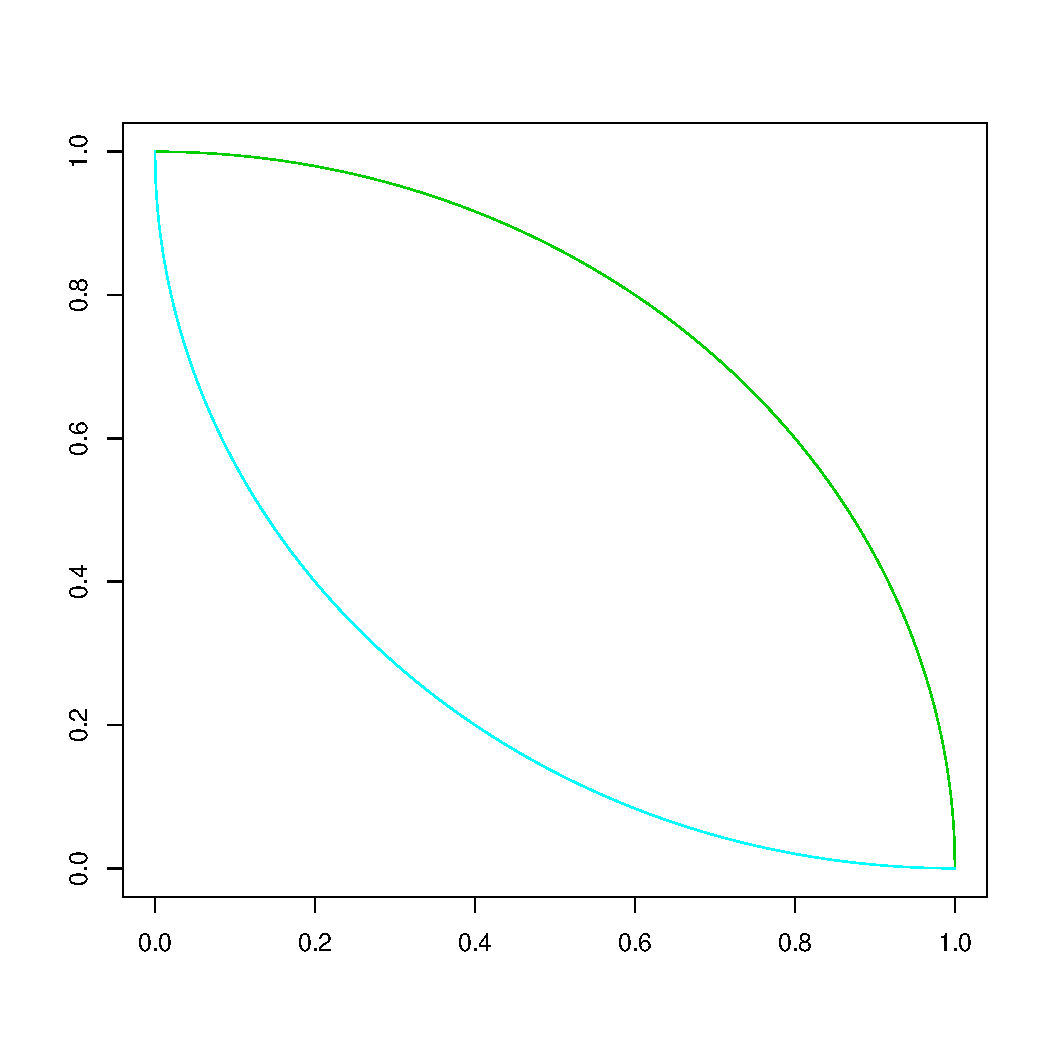
\includegraphics[width=150pt,angle=0.5]{dom.pdf}
\begin{center}
 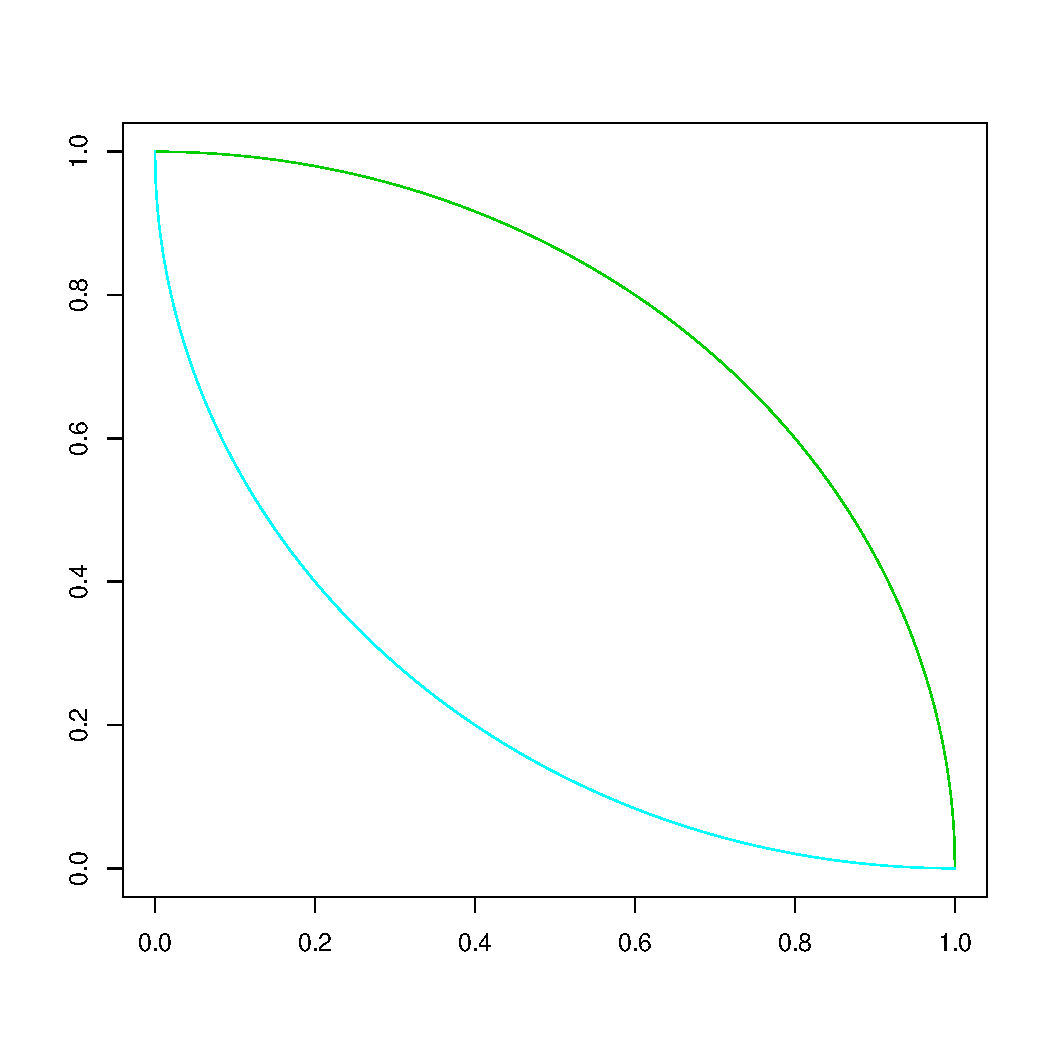
\includegraphics[scale=0.5]{dom.pdf}
\end{center}


\begin{enumerate}
 \item
      領域$D$は$[0,1]\times[0,1]$に含まれるが、
      点$(0,1),\,(1,0)$が$D$に含まれるので$I$はそれより大きく取る必要がある。

      例えば、$I=[-1,2]\times [-1,2]$と置けば、
      $D \subset (-1,2)\times (-1,2)$となる。

 \item
      $D$は縦線集合であるので、
      $D_{ij}$は$D$を$\Delta_{ij}$に制限する事により
      縦線集合として得られる。

 \item
      $C_1,\,C_2$を次のようにおく。
      \begin{align}
       C_1:& [0,1] \rightarrow \mathbb{R}^2, \quad x \to (x, \sqrt{1-x^2})\\
       C_2:& [0,1] \rightarrow \mathbb{R}^2, \quad x \to (x, 1-\sqrt{1-(x-1)^2})
      \end{align}
      この時、境界$D^b$は
      \begin{equation}
       D^b = \Img C_1 \cup \Img C_2
      \end{equation}

 \item
      $D$の分割$D_{ij}$は
      その境界を正の向きに向き付けすると、
      重なり合う部分は逆向きとなる。

      各$\partial D_{ij}$をつなぎ合わせると
      打ち消し合う境界が消え、向きづけされた$C_1,\,C_2$が残る。

      これにより
      向きづけされた境界$\partial D$が存在する。
\end{enumerate}

これらにより、
領域$D$は積分定理が利用できる領域である。

\hrulefill

\end{document}
